%%%%%%%%%%%%%%%%%%%%%%%%%%%%%%%%%%%%%%%%%%%%%%%%%%%%%%
%%%  Filename: template-proposal-thesis.tex
%%%  -------------------------------------------------
%%%  Template for Master Thesis Proposal at DTETI UGM   		
%%%  -------------------------------------------------
%%%  Written originally on MS Word by Harsoyo
%%%  
%%%  Convert to Latex by Agung Nugroho
%%%  agung.n2016@mail.ugm.ac.id
%%%  November 2018
%%%%%%%%%%%%%%%%%%%%%%%%%%%%%%%%%%%%%%%%%%%%%%%%%%%%%%

\documentclass[12pt]{article}
\usepackage{makeidx}
\usepackage{multirow}
\usepackage{multicol}
\usepackage[dvipsnames,svgnames,table]{xcolor}
\usepackage{graphicx}
\usepackage{epstopdf}
\usepackage{listings}        
\usepackage{ulem}
\usepackage{hyperref}
\usepackage{amsmath}
\usepackage{amssymb}
\usepackage{enumitem}
\usepackage[Indonesian]{babel} % english/Indonesian language/hyphenation

%to indent the beginning of every section
\usepackage{indentfirst}

%Gambar X.Y
% X adalah lokasi Bab
% Y adalah urutan gambar
\usepackage{chngcntr}
\counterwithin{figure}{section}

%\newcommand{\subsubsubsection}[1]{\paragraph{#1}\mbox{}\\}
%\setcounter{secnumdepth}{4}
%\setcounter{tocdepth}{4}

\title{}
\usepackage[paperwidth=595pt,paperheight=841pt,top=72pt,right=85pt,bottom=56pt,left=89pt]{geometry}

\makeatletter
	\newenvironment{indentation}[3]%
	{\par\setlength{\parindent}{#3}
	\setlength{\leftmargin}{#1}       \setlength{\rightmargin}{#2}%
	\advance\linewidth -\leftmargin       \advance\linewidth -\rightmargin%
	\advance\@totalleftmargin\leftmargin  \@setpar{{\@@par}}%
	\parshape 1\@totalleftmargin \linewidth\ignorespaces}{\par}%
\makeatother 

% new LaTeX commands


\begin{document}




\clearpage
\thispagestyle{empty}

\begin{center}
{ \LARGE \bfseries PROPOSAL PENELITIAN}\\[1.8cm]

{ \Large \bfseries JUDUL PROPOSAL TESIS HARUS DILETAKKAN DI SINI}\\[0.4cm]

\begin{figure}[!ht]
\centering

\includegraphics[width=195pt]{img-1.png}
\end{figure}

{ \large \bfseries Nama Mahasiswa Di Sini}\\[0.4cm]


{ \large \bfseries yy/xxxxxx/PTK/xxxxx}\\[1.4cm]

{ \large \bfseries Konsentrasi}\\[0.4cm]

{ \large \bfseries Sistem Isyarat Elektronis (contoh)}\\[2.4cm]

{ \large \bfseries PROGRAM STUDI MAGISTER TEKNIK ELEKTRO}\\[0.4cm]

{ \large \bfseries DEPARTEMEN TEKNIK ELEKTRO DAN TEKNOLOGI INFORMASI}\\[0.4cm]

{ \large \bfseries FAKULTAS TEKNIK}\\[0.4cm]

{ \large \bfseries UNIVERSITAS GADJAH MADA}\\[0.8cm]

\textbf{{\large November 2018}}
\end{center}
\pagebreak{}


\begin{center}

{ \large \bfseries HALAMAN PERNYATAAN}\\[2.4cm]

{ \large \bfseries Tesis ini adalah tema yang berasal dari}\\[0.4cm]

{ \large Dosen / Mahasiswa (pilih salah satu)}\\[1.4cm]

ttd\\[1.4cm]

{ \large \bfseries Nama Dosen : Dr. Arjuna Wiwaha (contoh)}\\[1.4cm]

{ \large Nama Dosen dan tanda tangan dosen harus ada jika Tesis berasal dari Dosen}\\[1.4cm]

{ \large \bfseries Proposal ini adalah karya sendiri. Semua sumber rujukan telah dikutip sesuai etika penulisan karya ilmiah.}\\[1.4cm]

{ \large \bfseries Tanggal : dd -- mm -- 20xx}\\[1.4cm]

ttd\\[1.4cm]

\uline{\textbf{\large Nama Mahasiswa}}

\textbf{\large Nomer Mahasiswa}
\end{center}
\newpage
\begin{center}
\section*{INTISARI}
\end{center}

Intisari adalah ringkasan yang sangat singkat proposal. Intisari tidak boleh lebih dari satu halaman. Paragraf pertama berupa latar belakang. Isikan latar belakang yang menjadi dasar adanya penelitian ini. Kata asing harus ditulis \textit{miring}.

Paragraf kedua berisi tujuan penelitian. Tuliskan tujuan secara singkat di paragraf ini.

Paragraf ketiga berisi metode yang direncanakan untuk mencapai tujuan penelitian.

Paragraf keempat berisi hasil penelitian. Namun karena tulisan ini masih proposal, maka hasil di intisari adalah hasil yang diharapkan atau masih berupa hipotesis. Jika sudah melakukan pendahuluan, maka hasil dapat berupa hasil pada penelitian pendahuluan tersebut, tetapi tetap harus ditambahkan hasil yang diharapkan pada penelitian keseluruhan.\\

\textbf{Kata Kunci} : Kendali \textit{Fuzzy}, Algoritma Genetik, \textit{Template Matching}, \textit{ANN}, minimal 4, kata maksimum 8 kata.
\pagebreak{}

\section{Pendahuluan}

\subsection{Latar Belakang}

Dokumen ini adalah template Proposal Penelitian Tesis Magister Teknik Elektro atau Teknologi Informasi FT UGM. Gunakan template ini untuk menulis proposal penelitian. Dokumen ini dapat diunduh dari situs web resmi Program Magister Teknik Elektro atau Teknologi Informasi FT UGM. 

Bagian Pendahuluan berisi Latar Belakang, Perumusan Masalah, Tujuan Penelitian, Manfaat Penelitian, Batasan Penelitian, dan Keaslian Penelitian.

Uraikan artikel-artikel yang menjadi latar belakang penelitian ini dilakukan. Tuliskan apa yang sudah dilakukan oleh peneliti lain. Referensi menggunakan cara IEEE. Kutipan diurutkan berdasar urut nomor \cite{metev1998}\cite{Breckling1989}. Urutan sitasi yang lebih dari satu yang berurutan dituliskan yang pertama dan yang terakhir saja \cite{metev1998}-\cite{Padhye1999}. Jika tidak berurutan harus ditulis semua [1][3][5].

Tidak disarankan ada gambar di bagian pendahuluan. Jika sangat diperlukan adanya gambar, maka harus sesuai ketentuan. Lihat di bab selanjutnya mengenai gambar.


%\hspace{15pt}{\normalsize \hspace{15pt} }
\subsection{Perumusan Masalah}

Perumusan masalah menjelaskan masalah yang ada sehingga penelitian perlu dilakukan. Diuraikan berdasarkan latar belakang penelitian yang sudah dijelaskan di sub sebelummnya. Perumusan masalah hanya berupa masalah, bukan apa yang dilakukan. Perumusan masalah biasanya bernada negatif yang perlu diselesaikan pada tujuan penelitian. Tidak ada sitasi. Bagian ini murni tulisan sendiri. 

\subsection{Tujuan Penelitian}

Judul bab atau subbab baru tidak boleh sendiri di bawah. Jika terpaksa sendirian di bawah, enter satu kali sehingga masuk halaman baru. 

Tujuan penelitian menerangkan apa yang ingin dicapai dari penelitian. Bagian ini adalah jawaban dari perumusan masalah yang diuraikan sebelumnya. Jika dimungkinkan, jelaskan ukuran keberhasilan dari penelitian yang akan dilakukan. Tujuan penelitian dapat lebih dari satu, namun tetap menjawab/menyelesaikan masalah. Jika tujuan penelitian lebih dari satu, tuliskan dengan \textit{bullet} atau \textit{numbering}. 


\subsection{Batasan Penelitian}
Jelaskan apa yang akan dilakukan dan apa yang tidak akan dilakukan dalam penelitian. Batasan juga dapat menjelaskan batasan alat, bahan, ataupun data penelitian. 

\subsection{Manfaat Peneltiian}
Jelaskan manfaat yang diperoleh jika penelitian berhasil. Jelaskan baik dari sisi ilmu pengetahuan maupun kemanfaatannya bagi masyarakat. Akan sangat baik jika ada manfaat bagi bangsa dan negara.

\subsection{Keaslian Penelitian}
Jelaskan \textit{novelty} atau kontribusi penelitian di sini. Uraikan dari latar belakang dengan lebih menonjolkan peran penelitian anda. Akan lebih banyak sitasi di sini dibandingkan di bagian latar belakang [4]-[7]. Jika ada kekurangan peneliti lain, sehingga proposal penelitian ini penting, ungkapkan di bagian ini.
 
\pagebreak{}



\section{Tinjauan Pustaka dan Landasan Teori}
Tempatkan bab baru di halaman baru. 

\subsection{Tinjauan Pustaka}
Jelaskan \textit{paper-paper} dan penelitian yang terkait  dengan penelitian anda di sini. Sitasi mungkin akan lebih banyak lagi di sini [1]. Penelitian-penelitian pendukung yang lebih banyak sebaiknya diungkapkan untuk memperjelas arah penelitian anda.  Penjelasan mengenai \textit{novelty} anda lebih banyak diuraikan lagi [8][9].
 
Uraikan  \textit{novelty} atau kontribusi penelitian dari keaslian penelitian dengan lebih detail di sini. Tonjolkan peran penelitian anda dengan menjelaskan penelitian yang sudah ada dengan gap penelitian yang akan diselesaikan. Akan lebih banyak sitasi [4]-[7]. Jika ada kekurangan peneliti lain, sehingga proposal penelitian ini penting, ungkapkan di bagian ini dengan lebih detail. 


\subsection{Landasan Teori}
Pada subbab ini dibahas mengenai dasar teori yang dipakai serta justifikasinya untuk menyelesaikan penelitian. Sitasi dari berbagai sumber, termasuk buku, web dan sumber yang lain dimungkinkan [8]-[10]. Tidak diperkenankan mengambil sumber yang tidak jelas asalnya, seperti blog pribadi dan/atau wiki [10]. Dasar teori yang mendasari penelitian termasuk rumus-rumus, algoritma yang akan dikembangkan, gambar, struktur diagram, dan lain-lain diungkapkan di sini. 

\subsubsection{Subbab yang Lebih Kecil}

Penulisan proposal dimungkinkan untuk membentuk subbab- subbab yang lebih kecil, namun disarankan untuk tidak lebih dari tiga poin angka, sebagaimana dalam contoh ini. Sebagai gantinya, subbab yang lebih dari tiga poin menggunakan huruf besar dan cetak miring.

%\begin{enumerate}[label=(\Alph*)]
%\item Gambar
%\subsubsubsection{Gambar}
\paragraph{\textit{A. Gambar}}\mbox{}

Setiap gambar harus diberi nomor dan diberi judul, sebagaimana terlihat dalam contoh Gambar 2.1. Setiap gambar harus ditunjuk di dalam narasi. Tidak hanya ditunjuk saja, namun gambar juga harus diterangkan makna gambar di dalam narasi.

Dalam contoh ini, Gambar 2.1 menjelaskan tentang sistem kontrol jaringan. Demikian seterusnya dijelaskan per bagian serta makna istilah-istilah di dalam gambar. \textit{Font} di dalam gambar harus seragam dan harus dapat dibaca dengan jelas. 

Jika terdapat lebih dari satu gambar, maka antara gambar yang satu dengan yang lain harus senada. Maksud senada adalah jenis dan besar \textit{Font} sama atau tidak jauh berbeda. Demikian juga dengan penggunaan garis, kotak dan lain-lain, harus sama atau hampir sama. 

\begin{figure}
\centering
 	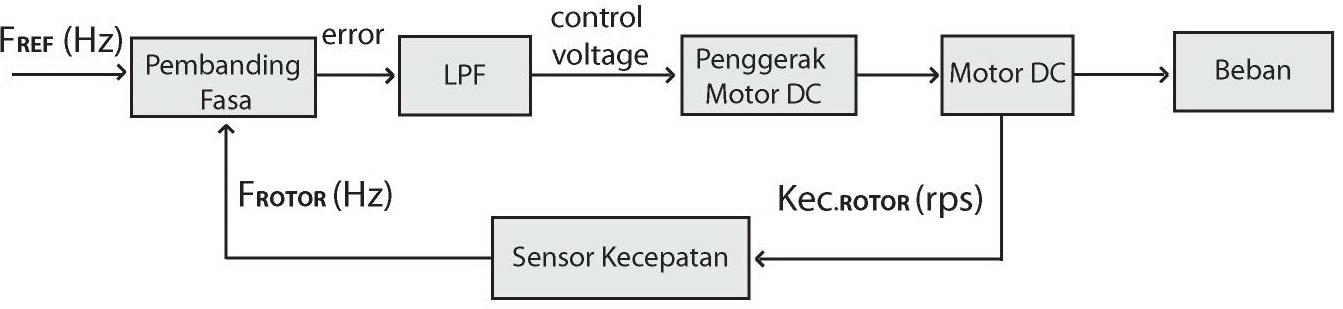
\includegraphics[width=1\textwidth]{img-2.png}
 	\caption{Sistem Kontrol Jaringan Terbuka (contoh)}  
\end{figure}
\pagebreak

%\paragraph{B. Grafik }

%\item Grafik
%\subsubsubsection{Grafik}

\paragraph{\textit{B. Grafik}}\mbox{}

Grafik merupakan gambar juga, sehingga ketentuan grafik sama dengan gambar. Baik pada gambar maupun grafik, gunakan ruang seperlunya agar tidak kelihatan berdesak-desakan.

Gambar 2.2 adalah contoh grafik. Jelaskan makna dari setiap istilah di dalam grafik. Jelaskan sumbu x, sumbu y, sumbu z (jika ada), serta makna setiap grafik yang ditampilkan. Angka-angka dan tulisan di dalam grafik harus dapat dibaca dengan jelas.


\begin{figure}[!ht]
\centering
 	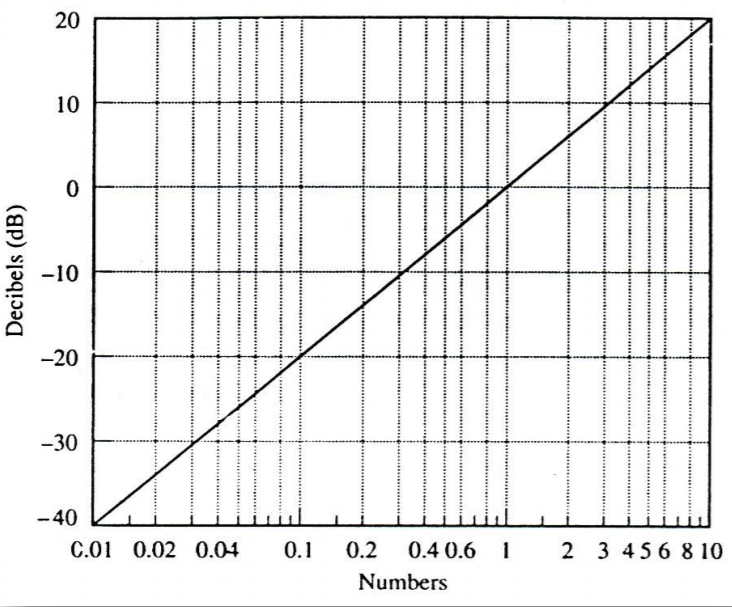
\includegraphics[width=0.6\textwidth]{img-3.png}
 	\caption{Garis Konversi Bilangan dB (contoh)[11]}  
\end{figure}

Dalam contoh ini, Gambar 2.2 menjelaskan tentang garis knversi bilangan dB. Demikian seterusnya dijelaskan per bagian serta makna istilah-istilah di dalam gambar. \textit{Font} di dalam gambar harus seragam dan harus dapat dibaca dengan jelas. 

Jika sebuah gambar/grafik diambil dari referensi tertentu, maka harus disebutkan sumbernya [11]. Usahakan agar letak gambar berada di bagian paling atas atau paling bawah halaman atau berada di akhir (sub) bab.

\pagebreak

%\paragraph{C. Tabel }

%\item Tabel
%\subsubsubsection{Tabel}
\paragraph{\textit{C. Tabel}}\mbox{}

Judul tabel diletakkan di atas dengan rata tengah (\textit{center}). Tabel 2.1 adalah contoh tabel. \textit{Font} dan penampakan tabel disesuaikan agar tabel tampak bagus dan mudah dibaca. Spasi \textit{single}. Tabel harus dirujuk di dalam narasi. Makna tabel, baik keterangan maupun nilainya harus dijelaskan. Disarankan letak tabel berada di bagian paling atas atau paling bawah halaman atau berada di akhir (sub) bab. Lakukan sitasi ketika sebuah tabel diambil dari referensi tertentu[12]. 

\begin{center}
{\small Tabel 2.1  Contoh Tabel [12]}

\vspace{3pt} \noindent
\begin{tabular}{|p{34pt}|p{142pt}|p{54pt}|p{54pt}|}
\hline
\parbox{34pt}{\centering 
\textbf{{\small No}}
} & \parbox{142pt}{\raggedright 
\textbf{{\small Keterangan}}
} & \parbox{54pt}{\centering 
\textbf{{\small Nilai 1}}
} & \parbox{54pt}{\centering 
\textbf{{\small Nilai 2}}
} \\
\hline
\parbox{34pt}{\centering 
{\small 1}
} & \parbox{142pt}{\raggedright 
{\small Uraian 1}
} & \parbox{54pt}{\centering 
{\small 1}
} & \parbox{54pt}{\centering 
{\small 2,3}
} \\
\hline
\parbox{34pt}{\centering 
{\small 2}
} & \parbox{142pt}{\raggedright 
{\small Keterangan 2}
} & \parbox{54pt}{\centering 
{\small 3}
} & \parbox{54pt}{\centering 
{\small 4,5}
} \\
\hline
\parbox{34pt}{\centering 
{\small 3}
} & \parbox{142pt}{\raggedright 
{\small Variabel}
} & \parbox{54pt}{\centering 
{\small 5}
} & \parbox{54pt}{\centering 
{\small 1,2}
} \\
\hline
\end{tabular}
\vspace{2pt}

\end{center}

%\end{enumerate}

\subsubsection{Kesalahan Yang Sering Terjadi}

Disarankan menggunakan kalimat yang lugas dan jelas. Hindari penggunaan anak kalimat yang berlebihan. Jika terpaksa ada anak kalimat, usahakan hanya satu anak saja. Penggunaan banyak anak kalimat atau bahkan beranak cucu akan membingungkan pembaca dalam menangkap maksud kalimat. Gunakan Bahasa Indonesia dengan baik dan benar.

Gunakan tata bahasa secara benar. Pastikan mana yang benar, di mana atau dimana, ke dua atau kedua, dan lain-lain. Kesalahan tata tulis dan/atau tata bahasa yang banyak dan fatal dapat menyebabkan proposal ditolak. Kesalahan seperti ini tidak sepantasnya dilakukan mahasiswa pasca sarjana. 


\subsection{Hipotesis / Pertanyaan Penelitian (Pilih salah satu)}

Tuliskan hipotesis/pertanyaan penelitian anda berdasarkan tujuan penelitian yang ingin dicapai.

\pagebreak{}


\section{Metode Penelitian}

Metode penelitian membahas segala sesuatu yang dilakukan untuk mencapai tujuan. Bab ini minimal berisi alat-alat yang digunakan, baik \textit{hardware} maupun \textit{software}, bahan yang dipakai, dan langkah-langkah penelitian. 

\subsection{Alat Penelitian}

Sebutkan alat-alat yang dipakai. Jika diperlukan disertai dengan kegunaannya. Alat yang dipakai dalam penelitian ini adalah:

\begin{enumerate}
\item Komputer 2 buah. Komputer ini satu digunakan sebagai client dan satu sebagai server. dan seterusnya dan seterusnya.

\item Laptop
\item PHP MYSQL
\item MATLAB (semua alat di muka adalah contoh)
\end{enumerate}

\subsection{Bahan}
Sebutkan bahan penelitian yang dipakai. Anda harus dapat membedakan antara alat dan bahan. Alat adalah perangkat untuk mengolah bahan, sedangkan bahan adalah yang diolah. Data penelitian dapat dimasukkan sebagai bahan, atau dapat dibuat subbab tersendiri. Sebutkan ada berapa data, dan diambil dari mana dan/atau bagaimana cara memperolehnya.

\subsection{Cara Penelitian}
Sebutkan langkah-langkah penelitian yang akan ditempuh untuk meraih tujuan penelitian yang ingin dicapai (lihat Tujuan Penelitian di Bab 1). Ungkapkan dalam bentuk gambar \textit{flowchart}. Jelaskan maksud \textit{flowchart} anda. Gambar 3. 1 adalah contoh langkah-langkah penelitian.

\begin{figure}[!ht]
\centering
 	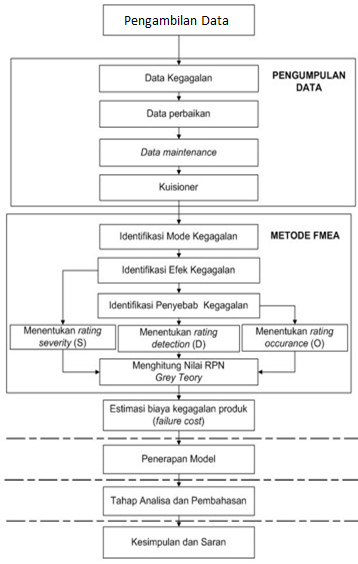
\includegraphics[width=1\textwidth]{img-4.png}
 	\caption{Langkah Penelitian (contoh)}  
\end{figure}

\pagebreak
Tidak perlu menyertakan studi literatur di dalam langkah penelitian. Studi literatur sudah jelas dilakukan pada setiap penelitian apapun. Jelaskan masing-masing tahapan pada Gambar 3. 1 yang dilakukan. Jelaskan tahapan-tahapan ini dalam subbab-subbab yang berurutan.

Selain langkah penelitian, gambar sistem yang dirancang perlu digambarkan. Gambar sistem harus disertakan ketika penelitian mengandung unsur perancangan sistem. Gambar 3. 2 adalah contoh gambar sistem.


\begin{figure}[!ht]
\centering
 	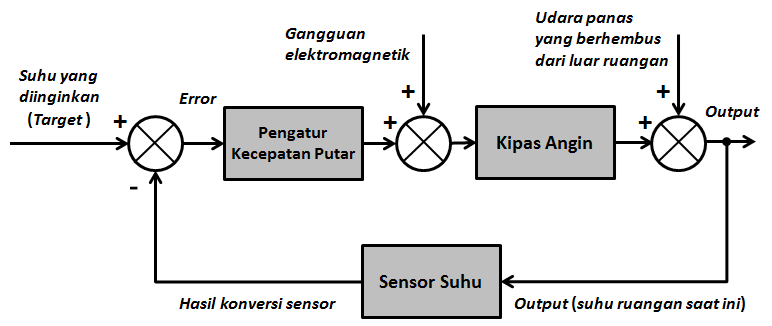
\includegraphics[width=1\textwidth]{img-5.png}
 	\caption{Gambar Sistem Penelitian (contoh)}  
\end{figure}


Gunakan simbol diagram yang tepat. Jelaskan makna Gambar 3. 2 secara keseluruhan, serta jelaskan makna masing-masing bagiannya.



\subsection{Hal Lain}
Ungkapkan hal-hal lain dalam penelitian jika dirasakan perlu. Hal-hal yang perlu diungkapkan mungkin saja berupa kesulitan-kesulitan, keterbatasan alat, kesulitan pengambilan data, dan lain-lain. Sebutkan bagaimana cara mengatasi atau skenario ketika gagal karena kesulitan/keterbatasan tersebut. Hal lain ini dapat juga berupa modal penelitian sebelumnya yang berhasil.

\pagebreak{}


\section{Jadwal Penelitian}
Ungkapkan jadwal penelitian anda dalam bentuk tabel. Penelitian dimulai sejak proposal disetujui dan mendapatkan dosen pembimbing. Jika proposal disetujui namun nama pembimbing belum ada, tanyakan ke Bagian Akademik atau Ketua Program Studi. Tabel 4. 1 adalah contoh Jadwal Penelitian. Sesuaikan dengan \textit{flowchart} yang dibuat di Metodologi (contoh Gambar 3.1). Apabila perlu, jelaskan jadwal yang dibuat.

\begin{center}
Tabel 4. 1 Jadwal Rencana Kegiatan Penelitian (contoh)
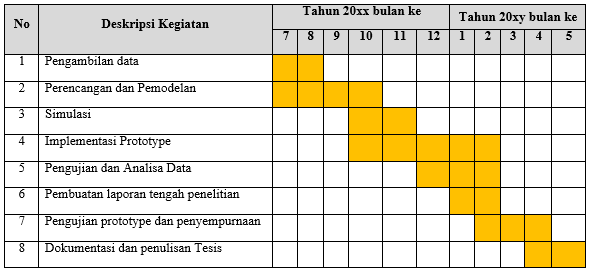
\includegraphics[width=372pt]{img-6.png}
\end{center}


\pagebreak{}

%Untuk menghilangkan tampilan garis bawah pada Title pustaka di daftar pustaka, digantikan dengan membuat teks Title pustaka menjadi teks miring.
\normalem
\bibliographystyle{ieeetran}
\bibliography{pustaka}





\end{document}